

If your architecture starts to look like spaghetti or you just want to prevent it, having your components structured in layers may help. Remember Model-View-Controller? Or maybe similar patterns, such as Model-View-ViewModel or Entity-Control-Boundary? Those are all typical examples of a layered architecture (also called N-tier architecture if the layers are physically separated from each other). You can structure code in layers, you can create layers of microservices, or apply this pattern to other areas where you think it could bring its benefits. Layering provides abstraction and the separation of concerns, and this is the main reason why it's being introduced. However, it can also help reduce complexity, while improving modularity, reusability, and maintainability of your solution.

A real-world example would be in self-driving cars, where layers can be used to hierarchically make decisions: the lowest layer would handle the car's sensors, then anothe layer would deal with single features consuming the sensor data, and on top of that one, there could be another one to ensure that all the features result in safe behavior. When sensors are replaced in another model of the car, only the lowest layer will need to be replaced.

A layered architecture is often pretty easy to implement since most developers already know the notion of layers – they simply need to develop several layers and stack them as in the following diagram: 

\begin{center}
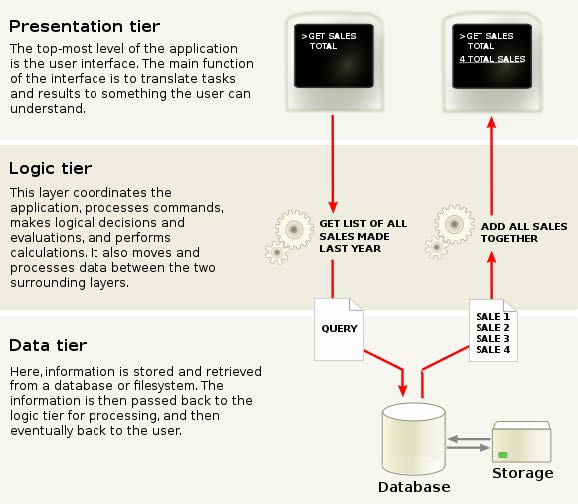
\includegraphics[width=0.9\textwidth]{content/1/chapter2/images/4.jpg}\\
Figure 2.4 – An example of a 3-tiered architecture using a textual interface in the presentation layer
\end{center}

The challenge with creating an efficient layered architecture lays in specifying stable, welldefined interfaces between the layers. Often, you can have several layers on top of one. For instance, if you have a layer for domain logic, it can be a base for a presentation layer and a layer for providing APIs to other services.

This doesn't mean that layering is always a good thing. With microservices, there are two main scenarios where layering emerges. The first is when you want to separate one group of services from another. For instance, you could have a fast-changing layer to engage with your business partners, with content that changes frequently, and another business capabilities-oriented layer. The latter is not being changed at such a fast pace and is using stable technologies. Separating those two makes sense. There's also a notion that less stable components should rely on more stable components, so it's easy to see that you could have two layers here with the customer-facing one depending on the business capabilities.

The other scenario is when layers are created to reflect the communication structure of the organization (hello again, Conway's law). This will probably reduce communication between the teams, which can result in a decrease in innovation as now the teams won't know the internals or ideas of each other that well.

Let's now discuss another example of a layered architecture often used with microservices—Backends for Frontends.



\subsubsubsection{2.6.1\hspace{0.2cm}Backends for Frontends}

It's not uncommon to see many frontends that rely on the same backend. Let's say you have a mobile application and a web application, both using the same backend. It may be a good design choice at first. However, once the requirements and usage scenarios of those two applications diverge, your backend will require more and more changes, serving just one of the frontends. This can lead to the backend having to support competing requirements, like two separate ways to update the data store or different scenarios for providing data. Simultaneously, the frontends start to require more bandwidth to communicate with the backend properly, which also leads to more battery usage in mobile apps. At this point, you should consider introducing a separate backend for each frontend.

This way, you can think of a user-facing application as being a single entity having two layers: the frontend and the backend. The backend can depend on another layer, consisting of downstream services. Refer to the following diagram:


\begin{center}
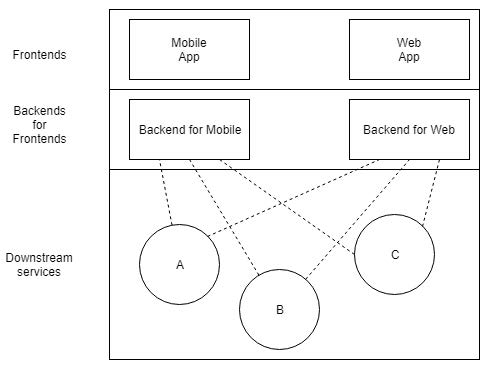
\includegraphics[width=0.9\textwidth]{content/1/chapter2/images/5.jpg}\\
Figure 2.5 – The Backends for Frontends pattern
\end{center}

The drawback of using \textbf{Backends for Frontends (BFFs)} is that some code must be duplicated. As long as this speeds up development and is not a burden in the long term, it's OK. But it also means that you should be on the watch for possibilities to aggregate duplicated logic in a downstream service. Sometimes, introducing a service just to aggregate similar calls can help solve duplication issues. Often, if you have many frontends, some can still share a backend and not cause it to have competing requirements. If you're creating mobile applications for iOS and Android, for instance, you could think of reusing the same backend for those, and having separate ones for web and/or desktop applications.






















